\documentclass[11pt]{article}
\usepackage[utf8]{inputenc}
\usepackage[T1]{fontenc}
\usepackage{lmodern}
\usepackage[a4paper,margin=1in]{geometry}
\usepackage{amsmath}
\usepackage{graphicx}
\usepackage{booktabs}
\usepackage{caption}
\usepackage[numbers,square,sort&compress]{natbib}
\usepackage{microtype}
\usepackage[hidelinks]{hyperref}
\hypersetup{pdftitle={Will It Load? What Decides Whether Agents Use On-Demand Skills},pdfauthor={Akshansh Gusain}}
\usepackage{url}

\captionsetup{font=small,labelfont=bf}
\newcommand{\code}[1]{\texttt{#1}}
\renewcommand{\bibfont}{\raggedright}

\title{Will It Load?\\ What Decides Whether Agents Use On-Demand Skills}
\author{Akshansh Gusain\\Independent researcher}
\date{November 2026}

\begin{document}
\maketitle

\begin{abstract}
Agent skills are increasingly loaded on demand: the agent sees only each skill's name and one-line description and must decide what to load. We study what decides that choice on ALFWorld, where every game has one relevant skill among five sibling skills and up to 300 distractors. A short instruction in the agent's prompt dominates. With an instruction to load a matching skill before acting, Claude Haiku 5.5 and DeepSeek V4.1 Flash load correctly at F1 0.80 to 0.98 across library sizes; without it, F1 falls to 0.00 to 0.18, and description wording, library size and naming change little. Errors are missed loads and confusions between sibling skills; distractors are almost never loaded. We then compare two description optimisers with identical inputs, one of which adds a persistent WikiSkill-style wiki of load evidence. Without the wiki, the optimiser learned imperative descriptions that raised Haiku's test F1 from 0.00 to 0.85 and 0.74 on two of three seeds, and the descriptions transferred to DeepSeek. With the wiki, Haiku's test F1 stayed at 0.00 on all seeds; its descriptions stayed almost entirely non-imperative, and in one seed its wiki recorded that wording was probably not the cause. Injecting 100 skills in full instead costs about 362k prompt tokens per call.
\end{abstract}

\section{Introduction}
\label{sec:intro}

Putting every skill in the prompt does not scale: with 100 realistic skills, each agent call carries about 362k prompt tokens. On-demand loading fixes the cost, but it moves the bottleneck to selection: the agent must notice and load the right skill from an index of names and descriptions.

Agent skills are reusable folders of instructions, scripts and resources. WikiSkill~\cite{tang2026wikiskill} evolves such skills from agent experience and keeps a persistent wiki of what it learns, so rejected attempts still leave lessons behind. Its executor sees the full text of every active skill in its prompt.

That design breaks as libraries grow. We measured it directly: 100 skills sampled from the SRA-Bench corpus~\cite{su2026sra} put about 362k tokens into every call of a Claude Haiku 5.5 executor. One SpreadsheetBench~\cite{ma2024spreadsheetbench} episode then cost \$0.10 on average (\$0.06 once the shared prefix was cached), against about \$0.002 with on-demand loading.

On-demand loading, as in the Agent Skills convention~\cite{anthropic2025overview,anthropic2025engineering}, shows the agent only each skill's name and description and lets it load a body when needed. The agent now has to decide what to load, and our probes show it often decides not to. With Haiku 5.5 as the executor, a relevant skill with a plain description was loaded on 9 of 10 tasks when alone, and on 0 of 10 once 20 or 100 unrelated skills sat beside it. Rewording only the description restored loading to 8 of 10 with 20 distractors.

The same kind of index behaves very differently elsewhere. In an ALFWorld~\cite{shridhar2021alfworld} pilot whose agent prompt told it to load a matching skill before acting, Haiku 5.5 loaded the relevant skill in 96\% of games with plain descriptions and 100 distractors. Loading is not a fixed property of a model. We ask what decides it: the agent's prompt, the wording of descriptions, the size of the library, how skills are named, and the executor. We then ask whether an optimiser that keeps a persistent wiki of load evidence, in the style of WikiSkill~\cite{tang2026wikiskill}, writes descriptions that get the right skills loaded.

Contributions:
\begin{enumerate}
\item A cost measurement: injecting 100 realistic skills in full costs about 362k prompt tokens per call.
\item A controlled study of what decides loading on ALFWorld, varying the agent's prompt instruction, description wording, library size from 20 to 300 distractors, descriptive versus opaque names, and two executors. The prompt instruction dominates: F1 0.80 to 0.98 with an instruction to load first, 0.00 to 0.18 without.
\item An error profile of loading: under the instruction, 2\% to 16\% of loads are sibling skills of the wrong type, and distractors appear among loads in only 2 of 28 settings.
\item A matched test of wiki-guided description optimisation. Without the wiki, the optimiser learned imperative descriptions that raised Haiku's test F1 from 0.00 to 0.85 and 0.74 on two of three seeds; with the wiki it stayed at 0.00, and its descriptions stayed almost entirely non-imperative.
\item A methodology note: load telemetry exposes accepted evolution edits that cannot be real gains, because the accepted skill was never loaded.
\end{enumerate}

\section{Related work}
\label{sec:related}

Prior work either evolves skill content with full injection, or improves selection with fixed components or trained weights. We found none that keeps a persistent, readable memory of why skills were or were not loaded.

\paragraph{Skill evolution.} WikiSkill~\cite{tang2026wikiskill} co-evolves skills with a persistent wiki and gates each edit on validation. Our work keeps WikiSkill's Maintainer, Proposer and gate, and points them at descriptions instead of bodies.

\paragraph{Skill retrieval at scale.} Skill Retrieval Augmentation~\cite{su2026sra} builds SRA-Bench: 5,400 test instances and a corpus of 26,262 skills, 636 of them gold. It finds that agents load skills at similar rates whether or not a gold skill was retrieved, and argues for utility-aware retrieval and for skills revised through agent self-improvement loops. We use its corpus as our distractor library.

\paragraph{Filtering retrieved skills.} Skill-V~\cite{ma2026skillv} represents skills as versioned, falsifiable contracts. It filters retrieved skills by applicability and revises a skill's boundary when contract checks disagree with task outcomes. It works on its own library and retrieval stack; we instead change the descriptions an agent sees in a standard Agent Skills index, and keep the selection evidence in a readable wiki.

\paragraph{Learned selection.} Skill1~\cite{shi2026skill1} trains one policy with reinforcement learning to select, use and distil skills. Selection ability ends up in the weights. Our method is training-free, works with closed models, and leaves its selection knowledge in readable wiki pages.

\paragraph{Progressive disclosure.} The Agent Skills convention~\cite{anthropic2025overview,anthropic2025engineering} lists skills by name and description and loads bodies on demand. We adopt its index format as our default, so our results describe a setup practitioners already use.

\section{Problem setup}
\label{sec:setup}

A skill is useful only if it is loaded on the tasks it serves and skipped on the rest. We score loads against known relevance, separately from task success.

\paragraph{Library and index.} The library holds $K$ target skills plus $N$ distractor skills. The executor never sees bodies up front. It sees a \code{load\_skill} tool whose description lists every skill as a name and a one-line description, in the Agent Skills format~\cite{anthropic2025overview,anthropic2025engineering}, and it may call the tool any number of times.

\paragraph{Ground truth.} In ALFWorld every game has one of six task types: look at an object in light, pick and place, clean then place, cool then place, heat then place, and pick two and place. We write one target skill per type. The relevant skill for a game is the skill for its type. The other five are near-miss siblings, and the $N$ distractors are sampled from the SRA-Bench corpus~\cite{su2026sra}.

\paragraph{Load-only episodes.} In our probes every load happened on the first turn. We therefore stop an episode at the agent's first environment action, or after five turns, and record every \code{load\_skill} call in order. This makes a selection measurement far cheaper than a full game; we report the measured cost per episode.

\paragraph{Metrics.} Over a set of games:
\begin{itemize}
\item Recall: share of games where the relevant skill was loaded.
\item Precision: share of all loads that were the relevant skill.
\item F1: harmonic mean of recall and precision.
\item Wrong-type rate: share of loads that were a sibling skill.
\item Noise-load rate: share of loads that were a distractor.
\end{itemize}
\begin{equation}
F_1 = \frac{2 \cdot \mathrm{Precision} \cdot \mathrm{Recall}}{\mathrm{Precision} + \mathrm{Recall}}
\end{equation}
Recall alone rewards loading everything, so the sibling skills matter: a description that grabs every game raises recall and costs precision.

\paragraph{Factors.} We vary five things and hold the rest fixed.
\begin{itemize}
\item Agent prompt: forced, which names the tool and tells the agent to call \code{load\_skill} for the matching skill before acting, or neutral, which mentions neither loading nor skills. In both, the index lives only in the tool description.
\item Descriptions: plain or directive.
\item Library size: 20, 100 or 300 distractors.
\item Names: the type names, or opaque names \code{skill\_01} to \code{skill\_06}, so that only the descriptions carry meaning.
\item Executor: Claude Haiku 5.5 or DeepSeek V4.1 Flash.
\end{itemize}

\section{Study design}
\label{sec:design}

Two experiments are fixed in advance, with a decision rule between them, so every outcome is reported rather than redesigned around.

\paragraph{Fixed skills.} Claude Sonnet 5.5 wrote one body per task type once, from general ALFWorld knowledge, with When to Apply, When NOT to Apply and Instructions sections, 19 to 20 lines per body. The bodies are hashed and never change. Two fixed description sets were written once: plain (``Procedure for heating an object and then putting it somewhere.'') and directive (``Load this before acting on any task that requires heating an object.'').

\paragraph{Experiment 1: what decides loading.} Load-only episodes on 60 validation games, 10 per task type, one pass per cell. Grid A crosses agent prompt (forced, neutral), descriptions (plain, directive), library size (20, 100, 300 distractors) and executor (Haiku 5.5, DeepSeek V4.1 Flash) with descriptive names: 24 cells. Grid B adds opaque names under the neutral prompt at 100 distractors: 4 cells.

\paragraph{Decision rule.} Among Haiku cells with the neutral prompt, we pick the one with the lowest plain F1 in which directive F1 exceeds plain F1 by at least 0.10, so that wording measurably matters. Ties go to the larger library, then to descriptive names. If no cell qualifies, Experiment 2 is not run and we report that selection left no room to optimise.

\paragraph{Experiment 2: wiki-guided description optimisation.} In the chosen cell, two optimisers start from the plain descriptions and may edit only descriptions. Each iteration runs 120 training games, the Proposer suggests new descriptions, and the candidate is kept only if F1 on the 60 validation games strictly improves. Each arm runs six iterations with three seeds, and each seed's baseline validation run is shared by both arms. The executor is Haiku 5.5 and the optimiser is Sonnet 5.5. Table~\ref{tab:arms} lists what each Proposer sees.

\begin{table}[t]
\centering
\caption{What the Proposer sees in each arm of Experiment 2.}
\label{tab:arms}
\begin{tabular}{lcc}
\toprule
What the Proposer sees & nowiki & wikisel \\
\midrule
Current descriptions and the fixed bodies & Yes & Yes \\
Per-skill training recall and precision & Yes & Yes \\
Every past candidate with its verdict, validation F1 & & \\
\quad and per-skill validation recall and precision & Yes & Yes \\
Wiki pattern pages written by a Maintainer & No & Yes \\
\bottomrule
\end{tabular}
\end{table}

The wikisel Maintainer, also Sonnet 5.5, reads eight sampled training traces per iteration. Each trace shows the task, the relevant skill, the loads in order, and the six target skills as the executor saw them, plus any distractor that was loaded. It writes selection-pattern pages in WikiSkill's wiki-edit format~\cite{tang2026wikiskill}, and the wiki is never rolled back. The two Proposer prompts are identical apart from one sentence telling wikisel where its wiki is.

\paragraph{Test.} After all runs finish, the final descriptions of every run, plus plain and directive, are scored on the 134 \code{valid\_unseen} games with one fixed distractor order: twice with Haiku 5.5, and once with DeepSeek V4.1 Flash as a transfer check. All calls go through OpenRouter with prompt caching on the static prefix and low reasoning effort.

\section{Preliminary findings}
\label{sec:prelim}

Five pilot results motivate the design: on SpreadsheetBench, loading collapses with distractors and wording rescues it; full injection is the expensive alternative; validation gains can be accepted for skills nobody loaded; load evidence changes what an optimiser edits; and on ALFWorld, an instruction to load may prevent the collapse.

\paragraph{Loading collapses, and wording is the lever.} We placed one relevant, generic spreadsheet workflow skill in an Agent Skills index, alone or among SRA-Bench distractors, on 10 training tasks. The body was identical in both styles; only the description changed. Plain: ``Workflow for spreadsheet manipulation tasks\ldots''. Directive: ``Use this skill for any task that reads or writes an .xlsx workbook. Load it before inspecting the file\ldots''. Table~\ref{tab:pilot} shows the result.

\begin{table}[t]
\centering
\caption{SpreadsheetBench pilot: tasks, out of 10, on which the relevant skill was loaded.}
\label{tab:pilot}
\begin{tabular}{lrcc}
\toprule
Executor & Distractors & Plain: loaded & Directive: loaded \\
\midrule
Haiku 5.5 & 0 & 9/10 & 10/10 \\
Haiku 5.5 & 20 & 0/10 & 8/10 \\
Haiku 5.5 & 100 & 0/10 & 1/10 \\
\midrule
Sonnet 5.5 & 0 & 7/10 & 10/10 \\
Sonnet 5.5 & 20 & 0/10 & 10/10 \\
Sonnet 5.5 & 100 & 0/10 & 8/10 \\
\bottomrule
\end{tabular}
\end{table}

Neither model loaded a distractor in 120 episodes, including the spreadsheet-related distractors in the library. Every load happened on the first turn. When the skill was skipped, the first action went straight to the workbook with no reasoning about the index.

\paragraph{Full injection is the expensive alternative.} With the same 100 distractors injected in full, Haiku 5.5 calls averaged 362,070 prompt tokens, all above the provider's 100k-token price tier, at \$0.10 per episode on average. One evolution run at that rate would cost \$76 to \$105 in executor calls alone.

\paragraph{Accepted without being loaded.} In seed-0 evolution runs with on-demand loading, 100 distractors and Haiku 5.5 as both executor and optimiser, the WikiSkill gate accepted five skill candidates across three arms. Every one had a validation load rate of 0/40: the executor never read the body it was credited for. The three arms shared an identical empty starting state yet differed by one task at baseline (0.775 vs 0.750), comparable to the accepted gains of one to two tasks.

\paragraph{Evidence changes the optimiser; instruction alone does not.} In those runs, an arm told only that skills load on demand kept the same description through five proposals, editing just the unread body. The arm that also saw load rates rewrote its description twice, into imperative and more specific wordings, then restored the original and added a second skill whose description began ``MUST load before''. With Haiku at 100 distractors none of the wordings were loaded.

\paragraph{An instruction to load may prevent the collapse.} In an ALFWorld pilot whose agent prompt said to call \code{load\_skill} for the matching skill before acting, Haiku 5.5 with 100 distractors loaded the relevant skill in 95.8\% of games with plain descriptions and 99.2\% with directive ones (F1 0.950 and 0.967, over 60 validation games and two passes). No distractor was loaded; the errors were loads of sibling skills. The SpreadsheetBench probe had no such instruction, and Experiment 1 tests this difference directly.

\section{Results}
\label{sec:results}

The instruction to load decided whether skills were loaded; among optimisers, the one without the wiki recovered loading and the one with it did not.

\paragraph{What decides loading (Experiment 1).} Figure~\ref{fig:exp1} shows F1 of loads on 60 validation games, one pass per cell; Table~\ref{tab:exp1} in Appendix~\ref{app:exp1} lists every cell with its 95\% interval.
\begin{figure}[t]
\centering
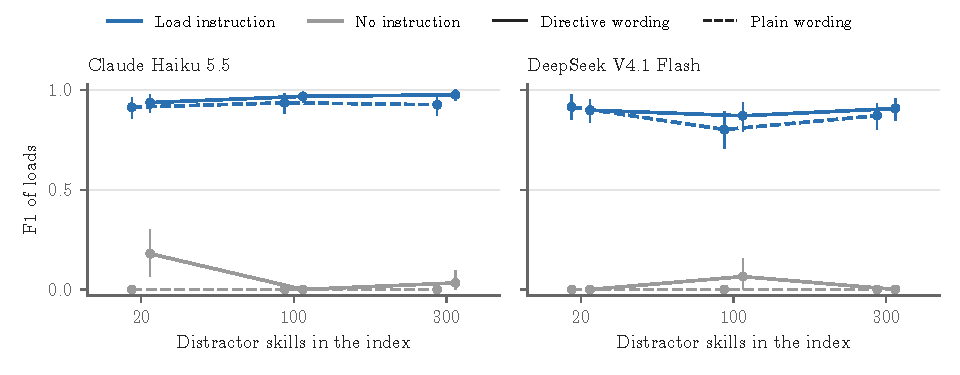
\includegraphics[width=\linewidth]{figures/fig1_exp1_f1.pdf}
\caption{F1 of loads in Experiment 1, on 60 validation games with descriptive skill names, one pass per cell. Blue: agent prompt with the load instruction (forced); grey: neutral prompt. Solid lines: directive descriptions; dashed: plain. Bars are 95\% bootstrap intervals over games. The four opaque-name cells (neutral prompt, 100 distractors) all scored F1 0.000 and are not drawn.}
\label{fig:exp1}
\end{figure}
With the instruction, both executors loaded well at every library size, and directive wording added at most 0.07 F1. Without it, they mostly acted on the first turn: no neutral cell had a load in more than 10\% of games. Opaque names gave no loads at all.

\paragraph{Errors.} Under the forced prompt, 2\% to 16\% of loads were sibling skills of the wrong type. Distractors appeared among loads in only 2 of 28 cells: 2.6\% of loads in one DeepSeek cell, and a single episode in another.

\paragraph{Decision.} One eligible cell met the rule: neutral prompt, descriptive names, 20 distractors, with plain F1 0.000 and directive F1 0.179. The other three eligible cells had gaps of 0.000 to 0.033. Experiment 2 ran in that cell.

\paragraph{Description optimisation (Experiment 2).} Figure~\ref{fig:exp2} shows validation F1 across iterations.
\begin{figure}[t]
\centering
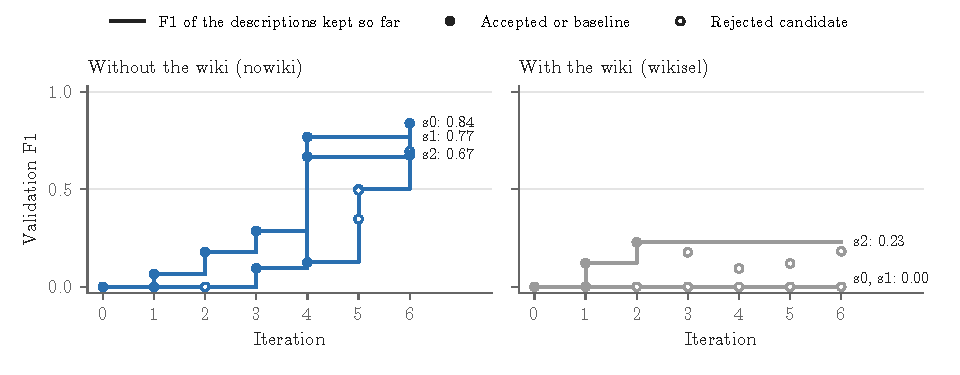
\includegraphics[width=\linewidth]{figures/fig2_exp2_val.pdf}
\caption{Validation F1 during description optimisation (Experiment 2): neutral prompt, descriptive names, 20 distractors, Haiku 5.5 executor, 60 validation games. Each line is one seed (s0--s2) and shows the F1 of the descriptions kept so far; filled dots are the baseline and accepted candidates, hollow dots are rejected candidates. Labels give each seed's final kept F1.}
\label{fig:exp2}
\end{figure}
Both optimisers started from the same history: per-skill recall of zero. nowiki responded by escalating the wording. We call a description imperative when it tells the agent to load the skill (``Load\ldots'', ``ALWAYS load\ldots'', ``MUST load\ldots''); one that begins ``Use when'' only says when the skill applies. nowiki's description of the heating skill in seed 0 went from ``Use when the task says to put a HOT, heated, or warm object somewhere'' in iteration 1, through ``ALWAYS load when the task says `hot', `heat', `warm', `cook'\,'', to ``MUST load FIRST, before any action, whenever the task says `hot', `heat', `heated', `warm' or `cook'\,'' in iteration 6. In seed 0, wikisel's Maintainer read traces with no loads and wrote a page concluding: ``Wording is probably not the cause. Check the load mechanism before making more description edits.'' Its other 17 pages described semantic cues, such as missing the cleaning skill when a task says ``wet''. Across all six iterations its descriptions began ``Use when'' or ``Use for'', and none were loaded. In seed 1 none of wikisel's descriptions became imperative either; in seed 2, one of six did in iteration 2, and later candidates kept at most that one. In every nowiki seed, all six descriptions were imperative from iteration 2 on. A wiki arm with a different setup did adopt imperative wording in the SpreadsheetBench pilot (Section~\ref{sec:prelim}), so this outcome is not inherent to wikis.

\paragraph{Test and transfer.} Figure~\ref{fig:test} shows test F1 on the 134 \code{valid\_unseen} games, all with seed 0's distractor order.
\begin{figure}[t]
\centering
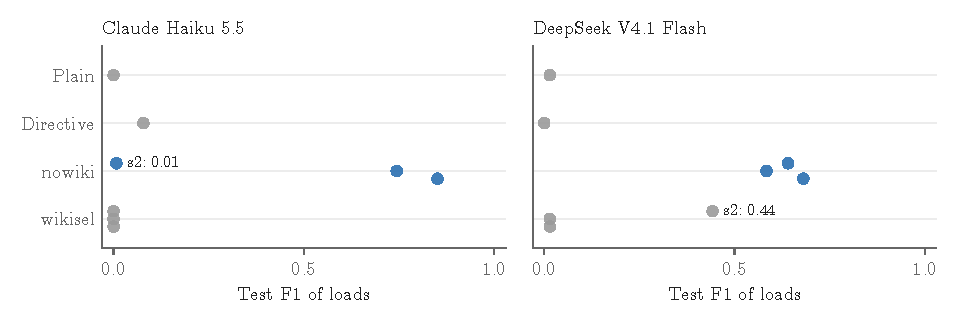
\includegraphics[width=\linewidth]{figures/fig3_test.pdf}
\caption{Test F1 on the 134 \code{valid\_unseen} games, with seed 0's distractor order for every evaluation. Each dot is one seed's final descriptions (plain and directive are fixed, so they have one dot); blue marks nowiki. Haiku 5.5 was scored over two passes, DeepSeek V4.1 Flash over one. Outlying seeds are labelled.}
\label{fig:test}
\end{figure}
Pooling all seeds and resampling games (10,000 draws), Haiku F1 differences are: nowiki minus plain $+0.620$ (95\% interval 0.584 to 0.653), nowiki minus directive $+0.542$ (0.482 to 0.595), and wikisel minus nowiki $-0.620$ ($-0.653$ to $-0.584$). With DeepSeek, nowiki minus plain is $+0.624$ (0.570 to 0.674) and wikisel minus nowiki is $-0.451$ ($-0.496$ to $-0.405$). nowiki's descriptions, learned with Haiku, held up on DeepSeek on all three seeds. nowiki's seed 2 did not hold up on Haiku's test: 0.674 on validation, 0.007 on test. The two seeds that held up wrote ``before any action'' in all six descriptions; seed 2 wrote it in none (see Section~\ref{sec:limits}).

\section{Limitations}
\label{sec:limits}

We measure whether the right skill is loaded, not whether loading it improves results, because at our scale no skill we tested improved task success.

\paragraph{No base effect at this scale.} We ran three checks before narrowing the question to selection.
\begin{itemize}
\item WikiSkill evolution on SpreadsheetBench with a Haiku 5.5 executor accepted no lasting skill, with either a Haiku or a Sonnet 5.5 optimiser. The one accepted skill scored 0.783 against 0.800 for the empty skill over three repeated validation passes.
\item Two frozen spreadsheet skills from an independent implementation~\cite{stahlg2026wikiskill}, fully injected, showed no detectable effect over three validation passes of 40 tasks. One is the skill it reports at +11.75 points, learned with a different model in a Codex-based harness: $-0.058$ for Haiku 5.5 (95\% interval $-0.125$ to 0.000; $-0.050$ after rescoring one rollout the harness failed to score) and $-0.008$ for DeepSeek V4.1 Flash ($-0.092$ to $+0.083$). The other showed no effect on Qwen 3.5 9B, DeepSeek V4.1 Flash or Haiku 5.5, though most Qwen rollouts never wrote a workbook at all.
\item A hand-written ALFWorld procedure skill showed no detectable effect on Haiku 5.5 ($+0.025$, interval $-0.025$ to $+0.083$) or DeepSeek V4.1 Flash ($-0.025$, interval $-0.083$ to $+0.033$).
\end{itemize}
Skills may be specific to the model and harness they were learned on. Our executors may also already know what generic skills tell them. By contrast, SkillsBench~\cite{li2026skillsbench} finds that curated skills raise average pass rates from 33.9\% to 50.5\% across 87 tasks, so our null results describe our setting, not skills in general.

\paragraph{Scope.} One benchmark with ground-truth relevance, two executors, Sonnet-written bodies held fixed, and three seeds at most. Experiment 1 uses one pass per cell, so the decision rule acts on single-pass estimates. The training split follows ALFWorld's own mix of task types, from 8 to 35 games per type. Validation sets of 40 to 60 tasks shift by one or two tasks between identical runs, so we rely on test sets and bootstrap intervals for claims. Whether these findings hold for other domains, executors and real skill libraries remains open. ALFWorld's human-written task texts can also disagree with a game's type label: Maintainers in two seeds flagged a training game typed pick and place whose text reads ``examine the statue with the lamp''. We kept the labels from the game folders.

\paragraph{Experiment 2 caveats.}
\begin{itemize}
\item The Maintainer prompt gives one example pattern name, \code{selection-missed-heat-\allowbreak when-microwave-\allowbreak mentioned}, which points towards semantic cues. It may have steered the wiki away from wording. We did not test a Maintainer prompt without that example.
\item wikisel's Proposer read the same files as nowiki's plus 17 to 19 wiki pages per seed. The extra reading may itself have diluted its attention to the per-skill load history; we did not test a wiki of matched length.
\item nowiki's seed 2 fell from 0.674 on validation to 0.007 on test. Seeds 0 and 1, which held up, wrote ``before any action'' in all six descriptions; seed 2 wrote it in none. Seed 2 was also evolved under its own distractor order but tested under seed 0's. We did not separate these causes.
\item Without the load instruction, loading sat near zero in almost every cell, so the effects of wording, library size and naming there are measured close to a floor.
\item Experiment 2 ran in one cell, with one executor during optimisation and three seeds per arm.
\item The test intervals resample games with all seeds pooled, so they capture variation over games, not variation between optimisation runs, which Figure~\ref{fig:test} shows is large.
\item The distractor descriptions come from a public corpus and are not written as commands. nowiki's imperative descriptions may work partly because they stand out among them; in a library where every description is imperative, the effect could shrink.
\end{itemize}

\paragraph{Compute.} We budgeted about \$50 of API calls for all experiments; the whole project used about \$33, of which the final experiment batch cost \$4.45. The budget ruled out evolving the full-injection arm with 100 distractors, at \$76 to \$105 per run (Section~\ref{sec:prelim}), so we report its measured cost instead.

\section{Conclusion}
\label{sec:conclusion}

Whether an agent loaded an on-demand skill depended less on the skill library than on a short instruction in the agent's prompt. With that instruction, two executors loaded the right skill reliably at every library size we tried; without it, they rarely loaded anything.

Descriptions can stand in for the missing instruction, but only when they are written as instructions. The optimiser without the wiki learned to write ``MUST load FIRST, before any action'' and, on two of three seeds, recovered most of the loss; its descriptions worked on a second executor too.

Adding a persistent wiki of load evidence made things worse here. Its wiki framed the failures as missed semantic cues, and in one seed concluded that wording was probably not the cause. The wiki is never rolled back, and in two of three seeds its optimiser never adopted imperative wording. Persistent experience is only as useful as the explanations it keeps: methods that never forget may also need a way to revise what they believe.

Imperative descriptions also raise a design question for open skill libraries: any skill author can tell the agent to load their skill first. Libraries that accept contributed skills may need a way to check or rank such claims.

\section*{Code, data and AI assistance}

The code, frozen skills, splits, prompts and all result files will be released at \url{https://github.com/akshanshgusain/odskill}. The experiment code was written with an AI coding assistant (Cursor), and the text was drafted with Claude (Anthropic). The author directed the study and is responsible for its content.

\bibliographystyle{unsrtnat}
\bibliography{refs}

\clearpage
\appendix
\section{All Experiment 1 cells}
\label{app:exp1}

Table~\ref{tab:exp1} lists every Experiment 1 cell: 60 validation games, one pass, noise shuffle seed 0. The F1 interval resamples games (10,000 draws, seed 0). Loaded-any is the share of games with at least one load of any skill. No episode errored.

\begin{table}[!h]
\centering
\caption{Experiment 1, every cell. R: recall; P: precision; WT: wrong-type rate; NL: noise-load rate; Any: loaded-any.}
\label{tab:exp1}
\small
\setlength{\tabcolsep}{3.5pt}
\begin{tabular}{llrllrrrcrrr}
\toprule
Prompt & Names & $N$ & Executor & Wording & R & P & F1 & F1 95\% CI & WT & NL & Any \\
\midrule
forced & descriptive & 20 & Haiku & plain & 0.967 & 0.866 & 0.913 & [0.855, 0.960] & 0.134 & 0.000 & 1.000 \\
forced & descriptive & 20 & Haiku & directive & 0.983 & 0.894 & 0.937 & [0.889, 0.976] & 0.106 & 0.000 & 1.000 \\
forced & descriptive & 20 & DeepSeek & plain & 0.967 & 0.868 & 0.915 & [0.851, 0.976] & 0.105 & 0.026 & 0.983 \\
forced & descriptive & 20 & DeepSeek & directive & 0.883 & 0.914 & 0.899 & [0.838, 0.952] & 0.071 & 0.000 & 0.900 \\
forced & descriptive & 100 & Haiku & plain & 0.967 & 0.906 & 0.935 & [0.880, 0.983] & 0.094 & 0.000 & 1.000 \\
forced & descriptive & 100 & Haiku & directive & 1.000 & 0.938 & 0.968 & [0.938, 0.992] & 0.062 & 0.000 & 1.000 \\
forced & descriptive & 100 & DeepSeek & plain & 0.767 & 0.839 & 0.801 & [0.708, 0.891] & 0.161 & 0.000 & 0.767 \\
forced & descriptive & 100 & DeepSeek & directive & 0.833 & 0.911 & 0.870 & [0.792, 0.938] & 0.089 & 0.000 & 0.850 \\
forced & descriptive & 300 & Haiku & plain & 0.933 & 0.918 & 0.926 & [0.872, 0.974] & 0.082 & 0.000 & 0.950 \\
forced & descriptive & 300 & Haiku & directive & 1.000 & 0.952 & 0.976 & [0.945, 1.000] & 0.048 & 0.000 & 1.000 \\
forced & descriptive & 300 & DeepSeek & plain & 0.783 & 0.981 & 0.871 & [0.800, 0.930] & 0.019 & 0.000 & 0.783 \\
forced & descriptive & 300 & DeepSeek & directive & 0.867 & 0.952 & 0.907 & [0.847, 0.958] & 0.048 & 0.000 & 0.867 \\
\midrule
neutral & descriptive & 20 & Haiku & plain & 0.000 & 0.000 & 0.000 & [0.000, 0.000] & 0.000 & 0.000 & 0.000 \\
neutral & descriptive & 20 & Haiku & directive & 0.100 & 0.857 & 0.179 & [0.063, 0.301] & 0.143 & 0.000 & 0.100 \\
neutral & descriptive & 20 & DeepSeek & plain & 0.000 & 0.000 & 0.000 & [0.000, 0.000] & 0.000 & 0.000 & 0.000 \\
neutral & descriptive & 20 & DeepSeek & directive & 0.000 & 0.000 & 0.000 & [0.000, 0.000] & 0.000 & 0.000 & 0.000 \\
neutral & descriptive & 100 & Haiku & plain & 0.000 & 0.000 & 0.000 & [0.000, 0.000] & 0.000 & 0.000 & 0.000 \\
neutral & descriptive & 100 & Haiku & directive & 0.000 & 0.000 & 0.000 & [0.000, 0.000] & 0.000 & 0.000 & 0.000 \\
neutral & descriptive & 100 & DeepSeek & plain & 0.000 & 0.000 & 0.000 & [0.000, 0.000] & 0.000 & 0.000 & 0.000 \\
neutral & descriptive & 100 & DeepSeek & directive & 0.033 & 1.000 & 0.065 & [0.000, 0.154] & 0.000 & 0.000 & 0.033 \\
neutral & descriptive & 300 & Haiku & plain & 0.000 & 0.000 & 0.000 & [0.000, 0.000] & 0.000 & 0.000 & 0.000 \\
neutral & descriptive & 300 & Haiku & directive & 0.017 & 1.000 & 0.033 & [0.000, 0.095] & 0.000 & 0.000 & 0.017 \\
neutral & descriptive & 300 & DeepSeek & plain & 0.000 & 0.000 & 0.000 & [0.000, 0.000] & 0.000 & 1.000 & 0.017 \\
neutral & descriptive & 300 & DeepSeek & directive & 0.000 & 0.000 & 0.000 & [0.000, 0.000] & 0.000 & 0.000 & 0.000 \\
\midrule
neutral & opaque & 100 & Haiku & plain & 0.000 & 0.000 & 0.000 & [0.000, 0.000] & 0.000 & 0.000 & 0.000 \\
neutral & opaque & 100 & Haiku & directive & 0.000 & 0.000 & 0.000 & [0.000, 0.000] & 0.000 & 0.000 & 0.000 \\
neutral & opaque & 100 & DeepSeek & plain & 0.000 & 0.000 & 0.000 & [0.000, 0.000] & 0.000 & 0.000 & 0.000 \\
neutral & opaque & 100 & DeepSeek & directive & 0.000 & 0.000 & 0.000 & [0.000, 0.000] & 0.000 & 0.000 & 0.000 \\
\bottomrule
\end{tabular}
\end{table}

\end{document}
